
\chapter{The Near Neutrino Detector: A Fine-Grained Tracker}
\label{ch:nd-nnd}

\section{Introduction} 
\label{sec:nd-nnd-intro}

The DUNE Fine-Grained Tracker (FGT) near detector consists of a straw-tube
tracking detector (STT) and electromagnetic calorimeter (ECAL) inside of a 0.4 T
dipole magnet. In addition, Muon Identifiers (MuIDs) are located in the
steel of the magnet, as well as upstream and downstream of the STT. The FGT
is designed to make precision measurements of the neutrino fluxes, 
cross sections, signal rates, and background rates. 
This document presents an overview of the FGT design, which 
will meet the physics goals and sensitivities of the DUNE experiment. 

\section{Motivation}
\label{sec:nd-nnd-motivation}

In order for DUNE to achieve the desired neutrino-oscillation sensitivity, the 
charged-current signal events
and neutral-current
background events in the DUNE far detector (FD) must be precisely 
predicted as a function of the parameters and variables that affect 
oscillations. These include energy, leading lepton (which tags the neutrino flavor) and the 
momentum and identification of particles generated by neutrino interactions. 
It is, therefore, crucial to measure the un-oscillated neutrino fluxes and 
their interactions at the near site. At the FD, the first and the second 
oscillation maxima signals occur at about 2.4 GeV and 0.8 GeV, respectively 
-- an energy regime where neutrino cross sections and fluxes have large 
uncertainties. 

In addition to the oscillation signal, it is 
critical to identify and measure processes such as neutral current $\pi^0$ production,
that can mimic oscillation signals 
at the FD. Thus, the principal focus of the neutrino detector will be 
on the neutrino-oscillation energy range of $E_\nu < 8$ GeV, as well as higher 
neutrino energies that produce background to the oscillation signal. Furthermore, the
$8<E_\nu < 20$ GeV energy range can be used as a ``control region'' or
as a region
to search for physics beyond the PMNS matrix. Clearly, 
the measurements must be 
comparable to those made in the FD, whose target material is liquid argon (LAr). 

Finally, the neutrino detector must measure nuclear effects, including
short-range correlations, twp-body currents, pion absorption, initial-state interactions, 
and final-state interactions. These nuclear effects 
have an impact on neutrino cross sections and energy determinations, and differences
between neutrinos and antineutrinos must be fully understood when searching
for CP violation.

The proposed detector will constrain the systematic uncertainties in the DUNE 
oscillation measurements. Regardless of the process under study, the 
systematic error should be less than the corresponding statistical error. 
The design presented here is the subject of study within the DUNE Science 
Collaboration. As these studies 
progress, the design of the DUNE Near Detector, 
referred to as the Fine Grained Tracker (FGT) in this document, may 
evolve from what is described here. 

\section{Overview of FGT Design}
\label{sec:nd-nnd-fgt}

A schematic drawing of the 
FGT design is shown in Figure~\ref{fig:STT_schematic}. 
The fine-grained tracker 
design will measure the neutrino-event rates and cross sections 
on argon, water, and other nuclear 
targets for both $\nu_e$ and $\nu_\mu$ charged current (CC) and
neutral current (NC) scattering events. Our FGT design 
consists of a STT, consisting of straw tubes, water targets, argon targets, 
and radiator targets, and an electromagnetic calorimeter inside of a
dipole magnet. In addition, muon detectors (MuID) consisting of resistive plate
chambers (RPCs) will be embedded in the steel
of the magnet. The FGT has excellent position and angular resolutions due to
its low-density ($\sim 0.1$ g/cm$^2$) and high-precision STT. This high 
resolution is important for determining the neutrino
vertex and determining whether the neutrino interaction occurs in the water
or argon target.  The
proposed $3.5\times3.5\times6.4$ m$^3$ STT will be positioned inside a 
dipole magnet with magnetic field, $B = 0.4$~T, for particle tracking.
The nominal active volume of the STT corresponds to 8~tonnes of mass.
Table~\ref{tab:comparison} summarizes the
performance for the FGT configuration, while
Table~\ref{tab:STT_specs} lists the requirements for the FGT.

With a 120-GeV proton beam, the neutrino event rates in the detector
will be $\sim~0.35\times 10^{-14}$ events/tonne/proton on target.
Assuming $0.5\times 10^{14}$ protons per beam spill, this corresponds
to $\sim 1.5$ events per spill in the 8~tonne active volume of the FGT
design.  Overlaps between interactions are expected to be
manageable thanks to the nanosecond-level timing of the FGT relative to
the $\sim 10 \mu$s beam spill length.

\begin{cdrfigure}[A schematic drawing of the fine-grained
tracker design]{STT_schematic}{A schematic drawing of the fine-grained
tracker design}
%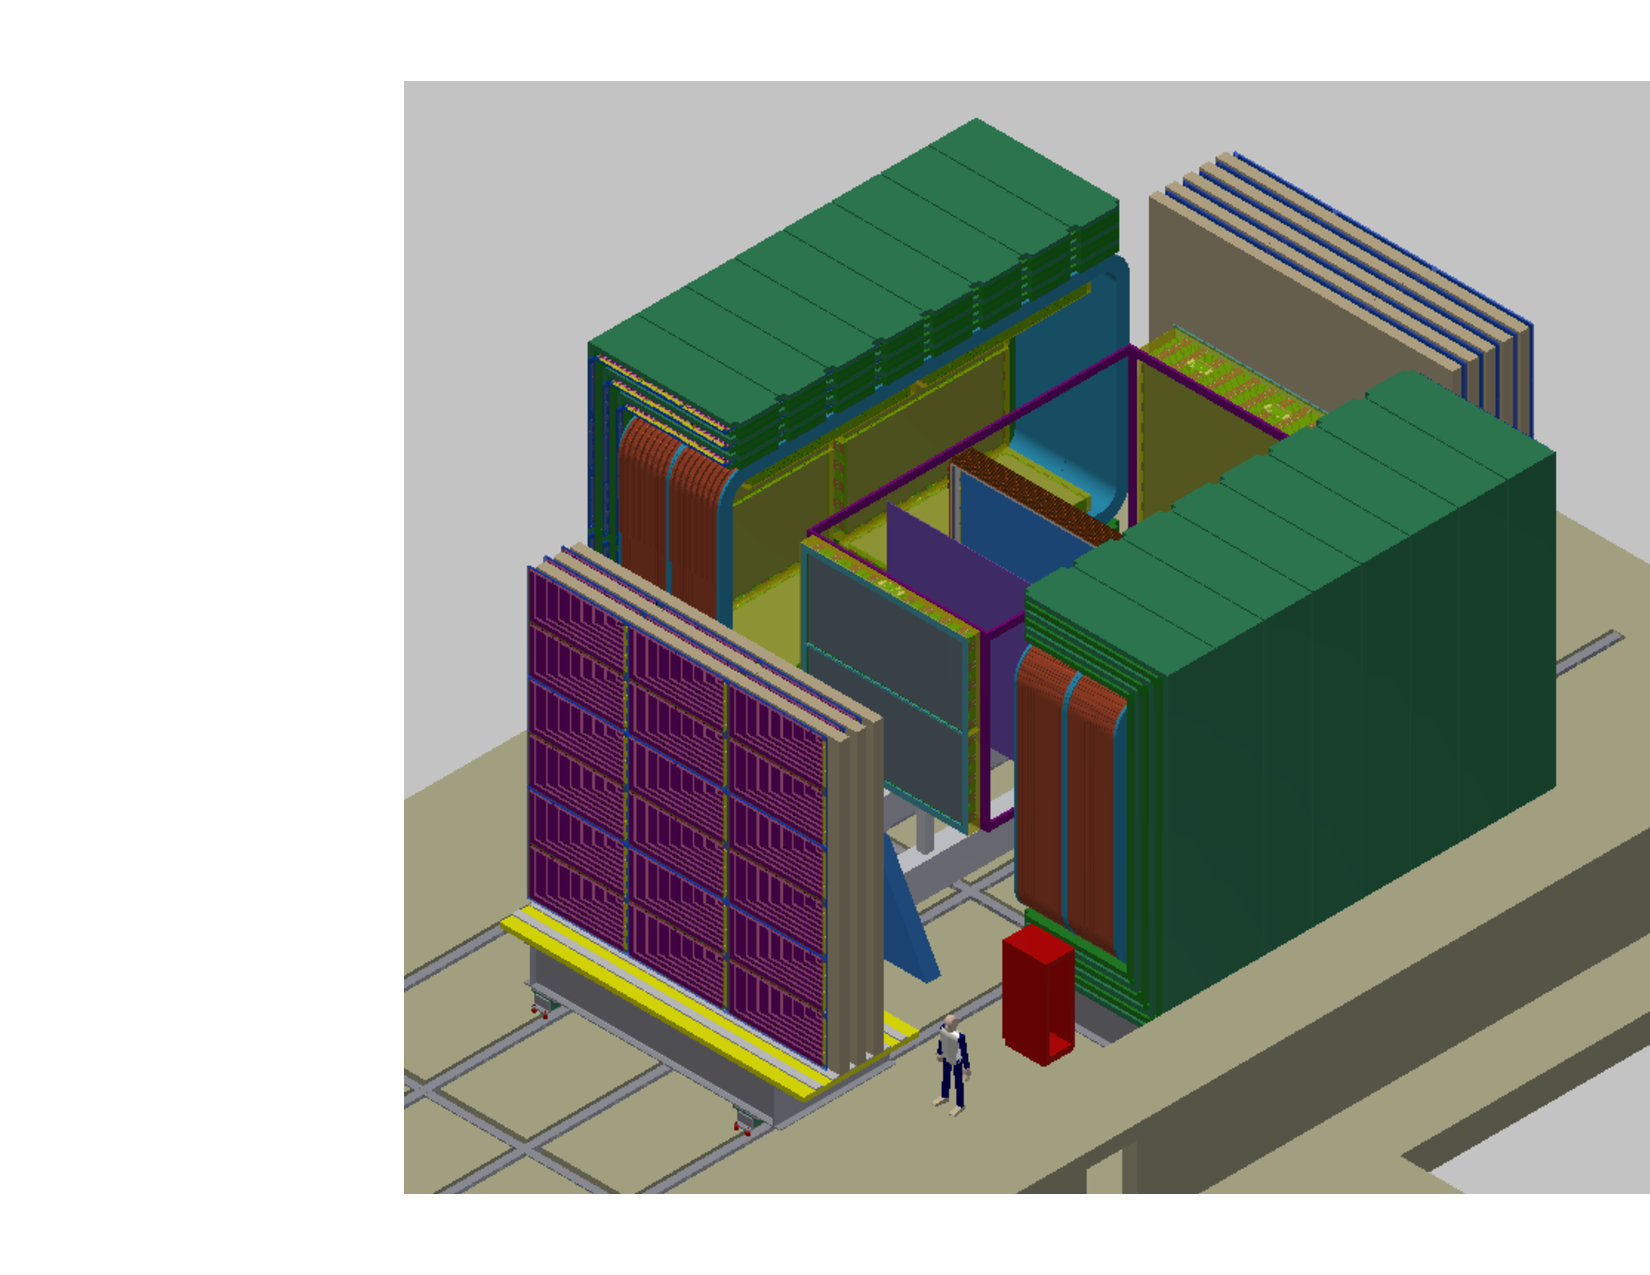
\includegraphics[width=5in,angle=90]{FGT_Overview}
\end{cdrfigure}



\begin{cdrtable}[A summary of the performance for 
the FGT configuration]{ll}{comparison}{A summary of the performance for 
the FGT configuration}
Performance Metric&FGT\\ \toprowrule
Straw Tube Detector Volume & 3.5m x 3.5m x 6.4m \\ \colhline
Straw Tube Detector Mass&8 tonnes\\ \colhline
Vertex Resolution&0.1 mm \\ \colhline
Angular Resolution&2 mrad \\ \colhline
$E_e$ Resolution&5\% \\ \colhline
$E_\mu$ Resolution&5\% \\ \colhline
$\nu_\mu/\bar \nu_\mu$ ID&Yes \\ \colhline
$\nu_e/\bar \nu_e$ ID&Yes \\ \colhline
NC$\pi^0$/CCe Rejection&0.1\% \\ \colhline
NC$\gamma$/CCe Rejection&0.2\% \\ \colhline
CC$\mu$/CCe Rejection&0.01\% \\
\end{cdrtable}


\begin{cdrtable}[Requirements for the FGT]{lp{8cm}}{STT_specs}{Requirements for the FGT}
Item&Requirement  \\ \toprowrule
Inner Magnetic Volume & 4.5m x 4.5m x 8.0m  \\ \colhline
Tracking Detector & 3.5m x 3.5m x 6.4m; 80 modules; 107,520 straws \\ \colhline
Targets & 1.27-cm thick argon, water, and other nuclear targets \\ \colhline
Transition Radiation Radiators & 3.6-cm thick radiators \\ \colhline
ECAL & $X_0$ = 10 barrel, 10 backward, \& 20 forward; 26,112 scintillator bars \\ \colhline
Dipole Magnet & 0.4T; 2.4 MW; 60 cm thick steel \\ \colhline
Magnetic Field Uniformity & $<2\%$ magnetic field variation over inner volume \\ \colhline
MuID & 432 RPC modules interspersed between 20-cm thick layers of steel \\  
\end{cdrtable}

\section{Straw Tube Tracking Detector}
\label{sec:nd-nnd-straw}

\subsection{Straw Tubes}

The STT is located at the center of the FGT and 
will be composed of straw tubes with an outer diameter of 1 cm, as well as 
radiators and targets. 
Vertical (YY) and horizontal (XX) planes of straws will be alternated and 
arranged in modules, with each module containing close-packed double straw layers 
of vertical and horizontal straws (XXYY). 
We have also considered an alternative design, which calls for two planes of straws
per module, XX, YY, so on. It will have approximately the same number of
total straw tubes in the tracker; however, the number of modules will be doubled.
In what follows, the performance and the cost of the STT is expected to be similar 
in the default (4-Planes/Module) and alternative (2-Planes/Module) designs.
The straw tubes will be filled with a
gas mixture of either 70\% Ar plus 30\% CO$_2$ (for modules with targets) or
70\% Xe plus 30\% CO$_2$ (for modules with radiators).
%A carbon composite sheet ($< 250 \mu$m thick), 
%as shown in Figure~\ref{STT_film}, 
%will provide support for each plane of straws. 
The dimensions of each module will
be approximately 350~cm $\times$ 350~cm $\times$ 8.0~cm, including 
target or radiator planes and four straw planes. For ease of construction and
transportation, each module is made up of six sub-modules, with dimensions of
appproximately 350~cm $\times$ 117~cm $\times$ 2.0~cm. 
The straw tubes in a single sub-module will be able to provide the tension 
for the wires; however, a temporary sub-module carbon composite frame will 
be employed for shipping. The sub-modules will be put together into modules 
at Fermilab, where each module will have a carbon composite frame around 
the perimeter of the module for support and will have an attached target or 
radiator. Nominally, there will be 34 modules with targets and 46 modules 
with radiators, still keeping the 
average density of the STT at around 0.1 g/cm$^3$. Figure~\ref{fig:STT_Detail}
shows a schematic drawing of a STT module with four straw-tube planes and
radiators.


\begin{cdrfigure}[A schematic drawing of a STT module]{STT_Detail}{A schematic drawing of a STT module with four straw-tube planes and
radiators (dark blue shading)}
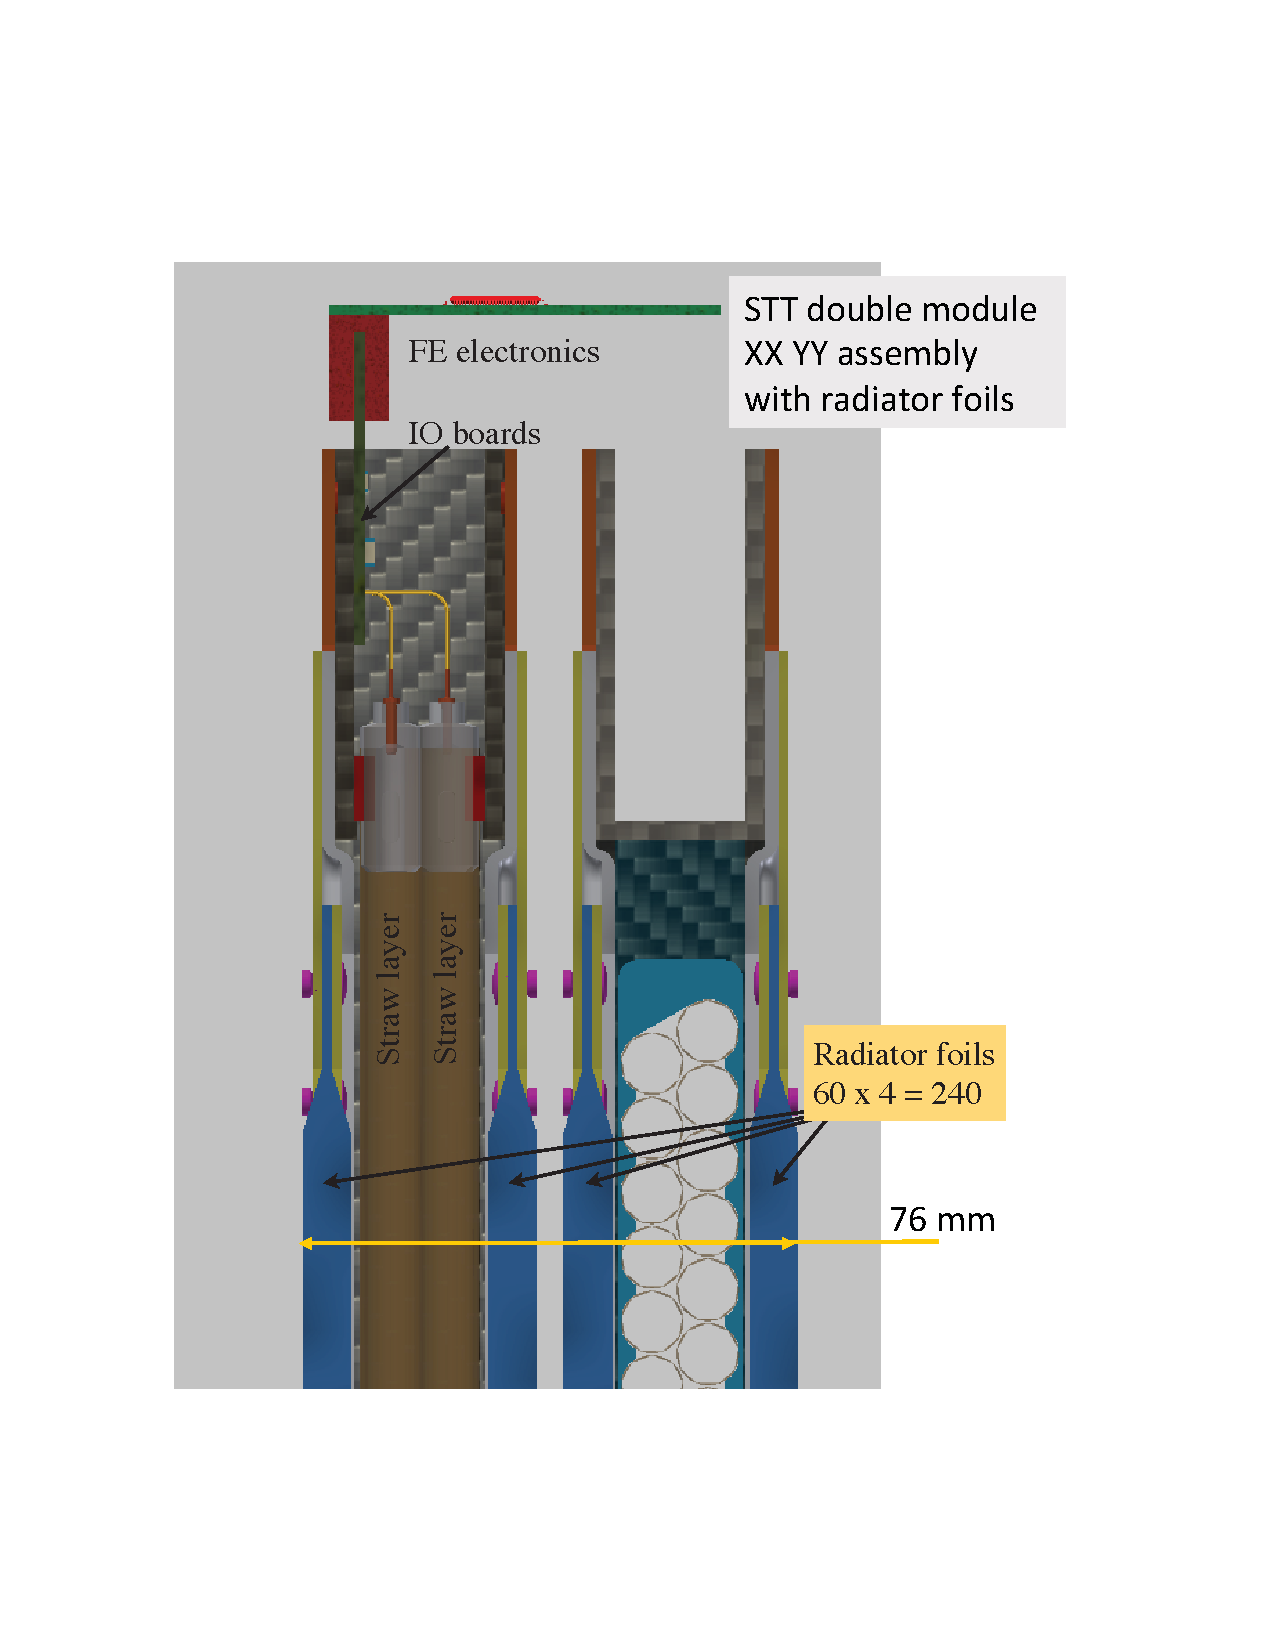
\includegraphics[width=4in,angle=90]{STT_Detail}
\end{cdrfigure}

There are a total of 107,520 straws, corresponding to 336 straws per plane,
1344 straws per module,
and 80 modules. Both ends of the straw tubes will be read out, so that the total
number of electronics channels will be 215,040. 
The total mass of the STT, including targets and radiators, is approximately 8 
tonnes, corresponding to an average density of 0.1. 
The thickness of the entire 6.4-m-long STT is almost two 
radiation lengths. Specifications for the Straw Tube Detector are shown in Table~\ref{tab:STT_details}.





\begin{cdrtable}[Straw Tube Detector specifications]{ll}{STT_details}{Straw Tube Detector specifications}
Item&Specification \\ \toprowrule
Straw Tube Geometry & 1cm Diameter x 3.5m Long \\ \colhline
Number of Straw Tubes & 107,520 \\ \colhline
Number of Straw Tubes per Plane & 336 \\ \colhline
Number of Straw Tube Planes per Module & 4 \\ \colhline
Number of Straw Tube Sub-Modules per Module & 6 \\ \colhline
Number of Straw Tube Modules & 80 \\ \colhline
Number of Straw Tube Sub-Modules & 480 \\ \colhline
Length of Straw Tube Wire & 376.3 km \\ \colhline
Number of Electronics Channels & 215,040 \\ \colhline
Number of Modules with Radiators & 46 \\ \colhline
Radiator Thickness per Module & 3.6cm \\ \colhline
Radiator Mass per Module & 108 kg \\ \colhline
Number of Modules with Target Planes & 34 \\ \colhline
Target Geometry & 1.27cm Diameter $\times$ 3.5m long \\ \colhline
Number of Targets per Plane & 275 \\ \colhline
Ar Mass per Plane & 15.5 kg \\ \colhline
Water Mass per Plane & 95 kg \\
\end{cdrtable}

\subsection{Radiator Targets}

Radiators will be placed in the downstream STT modules
and will serve as a target for both neutrino interactions 
and Transition Radiation (TR) production. Each STT module contains 
4 radiators, where each radiator consists of
60 layers of 25-$\mu$m polypropylene (C$_3$H$_6$)$_n$ 
%\fixme{the subscript 'n' is ok? yes} 
% Yes, 'n' is OK - BL
foils alternating with 60 sheets of 125-$\mu$m tulle fabric spacers. 
The mass of each radiator is $\sim 27$ kg and the thickness is 
$\sim 9$ mm. % AH rewrote pgraph a bit 
%The radiator accounts for about 85\% of the total mass
%of the module. 
Thin graphite planes and/or Carbon fiber foils can be added to some STT modules
in order to have a total C target mass of about 0.5 tonnes. (This is in addition to
the carbon in the STT frames.) A statistical subtraction of events occurring
on the pure C target from the ones in the polypropylene radiators will provide a measurement of
antineutrino interactions on a free proton target, which can be used for flux determination and cross-section
measurements.

\subsection{Argon, Water, \& Other Nuclear Targets}

We will implement both argon
and water as target materials for neutrino interactions.
The argon targets will measure neutrino interactions on the same material as the far detector, while
H$_2$O and D$_2$O water targets can be used to determine, through subtraction, the
neutrino fluxes off of ``free'' neutron targets. Antineutrino fluxes off of ``free''
proton targets can be obtained, through subtraction, from C and CH$_2$ targets.
The targets will be 
positioned directly upstream of individual modules without radiators. 
The targets, shown in 
Figure~\ref{fig:STT_targets}, will consist of planes of 0.5-inch diameter, 3.5-m-long aluminum tubes filled
either with water (H$_2$O or D$_2$O) or with argon gas pressurized to 140 atm ($\rho = 0.233$). 
%There will be a total of 44 modules 
%with argon targets and 20 modules with water targets. 
We will place 273 tubes in each 
plane, spaced 0.505-in apart. The tube wall thickness will depend on the fill material.
%; 0.065-in for the 
%pressurized Ar and 0.028-in for water. The water mass per plane is 95 kg 
%(106 kg for D$_2$O), 
%corresponding to a total water mass
%(H$_2$O and D$_2$O) of 1.9 tonnes. 
%while the argon mass per plane is 15.4 kg.
%, corresponding to a total argon mass of 0.68 tonnes.
Additional nuclear targets, such as Ca (same atomic weight as argon), C, stainless
steel, and Pb, can also be used in
the form of thin planes, to be positioned directly upstream of individual STT modules without radiators.


\begin{cdrfigure}[Schematic drawing of the water or pressurized-argon targets]{STT_targets}{Schematic drawing of the water or pressurized-argon targets, 
made from 0.5-in diameter aluminum tubes}
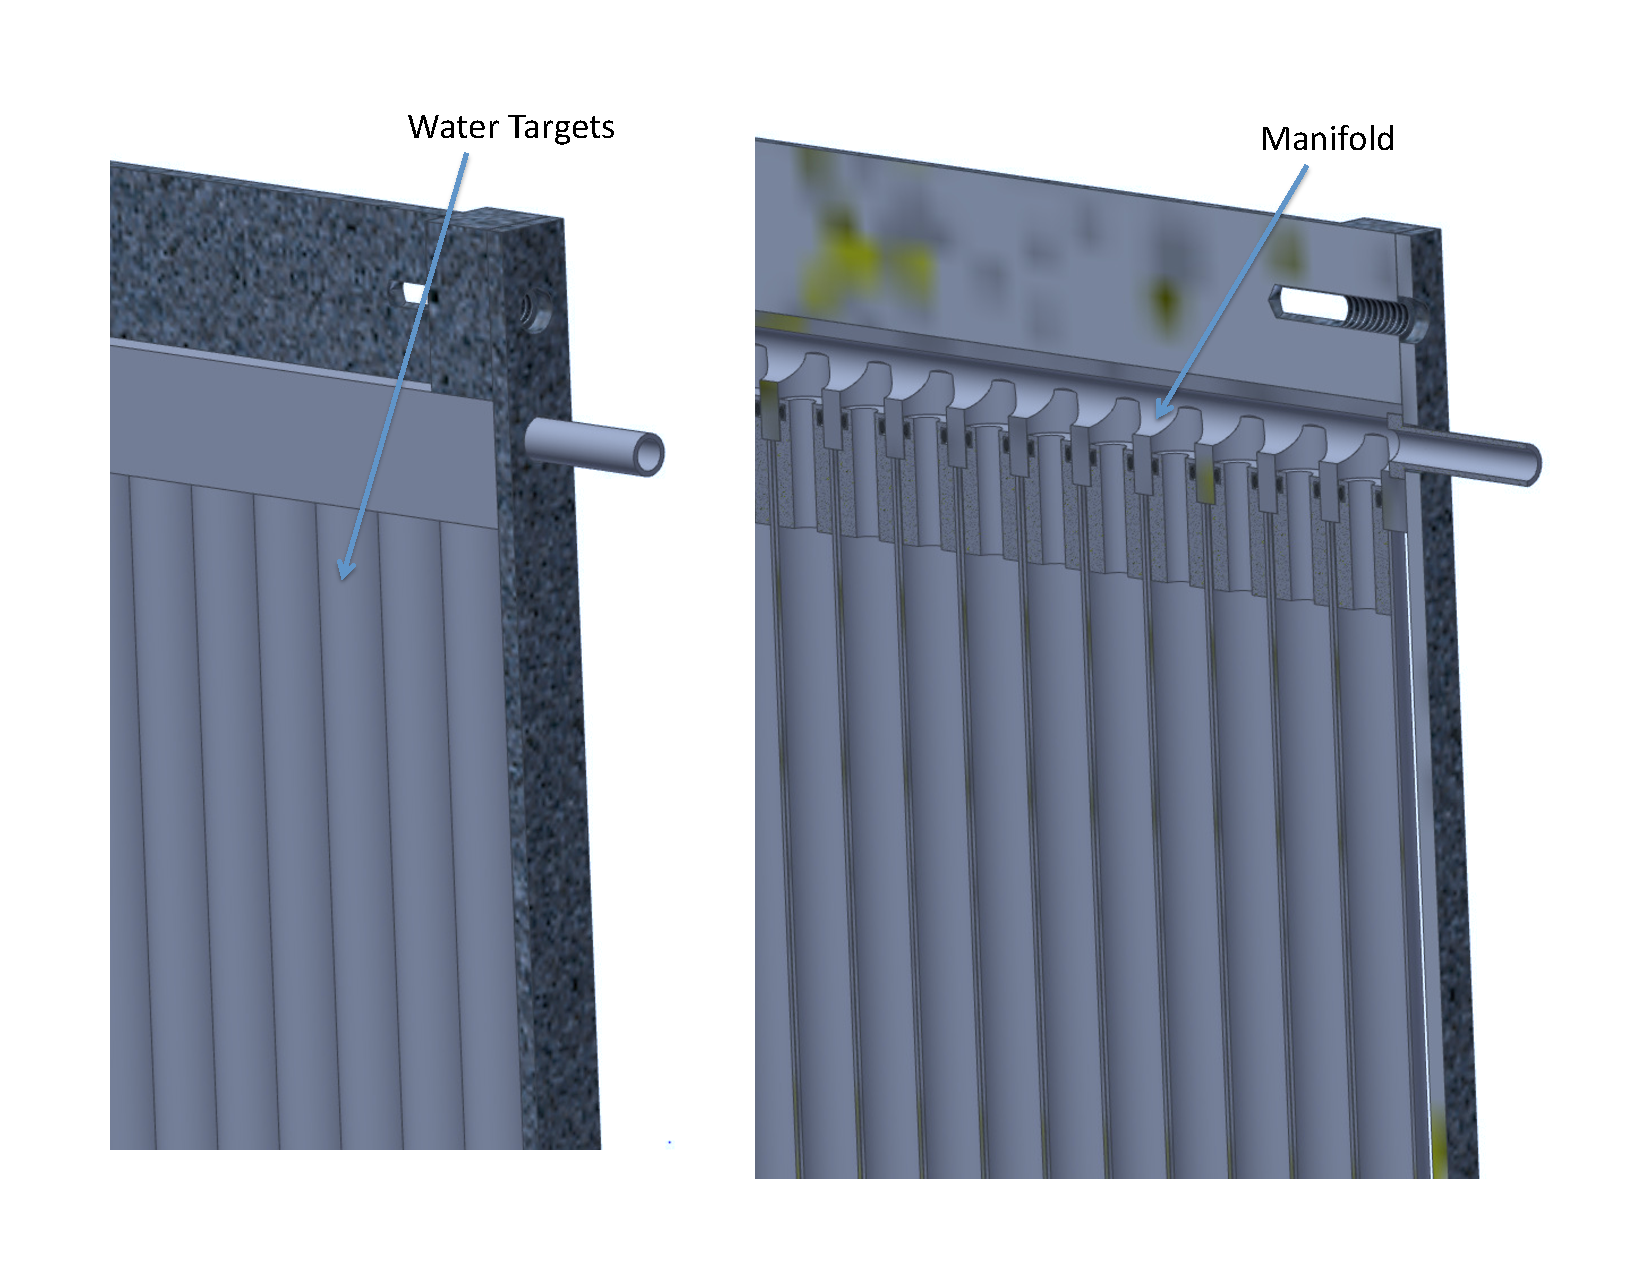
\includegraphics[width=4in,angle=90]{Water_target}
\end{cdrfigure}

\section{Electromagnetic Calorimeter}
\label{sec:nd-nnd-emcalo}

An electromagnetic calorimeter 
(ECAL) will surround the tracking volume on all sides and consist of three separate pieces: Forward ECAL, Barrel ECAL, and Backward ECAL. 
The ECAL conceptual design 
%is based on the design of the T2K ECAL and 
consists of 
layers of either 1.75-mm-thick (for the forward ECAL) or 3.5-mm-thick 
(for the barrel and backward ECAL) lead sheets and 2.5-cm-wide by 10-mm-thick 
plastic scintillator bars,
as shown in Figure~\ref{fig:ECAL_detail}. The scintillator layers for the
Forward and Backward ECAL alternate as XYXYXY..., while the scintillator 
layers for the Barrel ECAL are all horizontal along the axis of the magnet.
The Forward ECAL will consist of 60 layers of scintillator bars, where each
bar has dimensions 3.2~m $\times$ 2.5~cm $\times$ 1~cm. The
Backward ECAL will consist of 16 layers of scintillator bars, where each 
bar has the same dimensions, 3.2~m $\times$ 2.5~cm $\times$ 1~cm. The Barrel ECAL will also consist 
of 16 layers of scintillator bars, where each bar has the same dimensions, 
3.2~m $\times$ 2.5~cm $\times$ 1~cm. 

The lead sheets and scintillator bars will be assembled and glued together
into complete modules of dimension 3.2~m x 3.2~m x 81~cm for the Forward ECAL and
3.2~m x 3.2~m x 27.5~cm for the Backward ECAL. For the Barrel ECAL the module 
dimensions will be 3.2~m x 3.2~m x 27.5~cm. Two Barrel modules are placed end to
end along the sides of the inner surface of the magnet (8 Barrel modules
total) to provide full coverage of the barrel region.
The total numbers of scintillator bars in the
Forward, Backward, and Barrel ECAL are 7680, 2048, and 16,384, respectively, 
for a total of 26,112 bars. 

The scintillator bars will be extruded with 
holes in the middle of each bar. The
holes will then be fitted with 0.7-mm-diameter Kuraray wavelength-shifting (WLS) fibers.
The fibers will be read out by SiPM photosensors at each end, making the number of 
readout channels twice the number of scintillator bars 
for a total of 52,224. The total mass of scintillator is 20.9 tonnes, 
the total mass of Pb is 70.8 tonnes, and
the total length of fiber is 83.6 km.
Specifications for the ECAL are shown in Table~\ref{tab:ECAL_specs}, while 
Figure~\ref{fig:ECAL_gaps} shows a side view of the ECAL (red) inside the dipole
magnet, where there is very little gap between the Barrel ECAL and the Forward ECAL.


\begin{cdrfigure}[Schematic drawing of the ECAL]{ECAL_detail}{Schematic drawing of the ECAL, which is made up of alternating planes
of plastic scintillator and Pb sheets.}
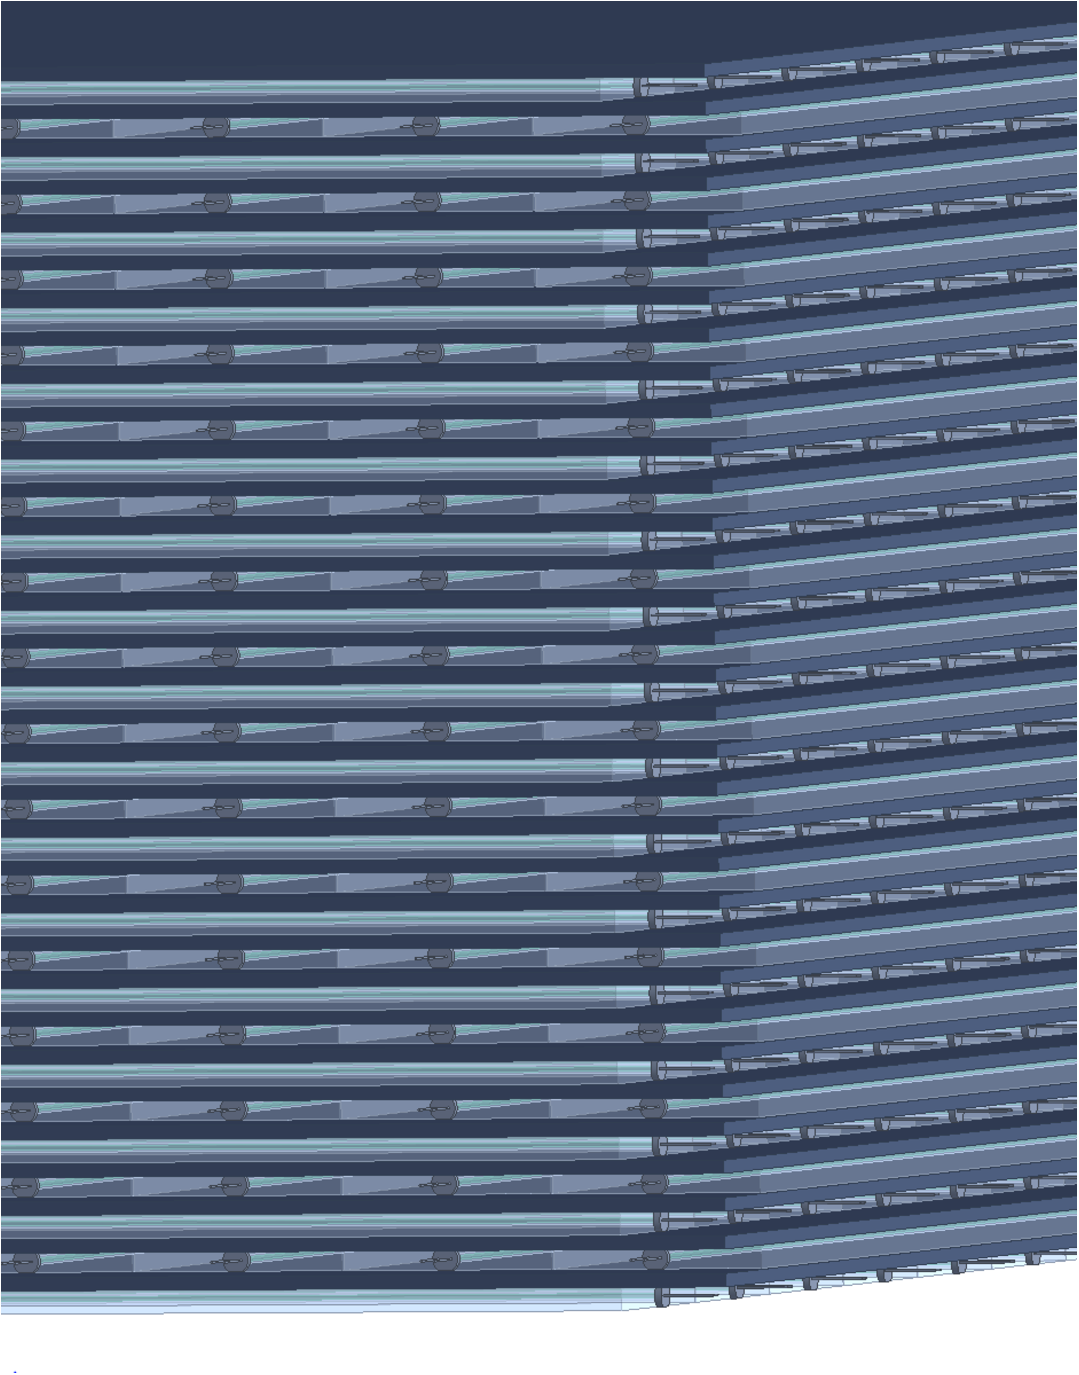
\includegraphics[width=3.0in,angle=90]{ECAL_detail}
\end{cdrfigure}



\begin{cdrtable}[ECAL specifications]{ll}{ECAL_specs}{ECAL specifications}
Item&Specification \\ \toprowrule
Scintillator Bar Geometry & 3.2m $\times$ 2.5cm $\times$ 1cm \\ \colhline
Number of Forward ECAL Scintillator Bars & 7680 \\ \colhline
Forward ECAL Pb thickness & 1.75mm \\ \colhline
Number of Forward ECAL Layers & 60 \\ \colhline
Number of Forward ECAL Radiation Lengths & 20\\ \colhline
Dimensions of Forward ECAL Module & 3.2m $\times$ 3.2m $\times$ 81cm \\ \colhline
Number of Barrel ECAL Scintillator Bars & 16,384 \\ \colhline
Barrel ECAL Pb thickness & 3.5mm \\ \colhline
Number of Barrel ECAL Layers & 16 \\ \colhline
Number of Barrel ECAL Radiation Lengths & 10 \\ \colhline
Number of Barrel ECAL Modules & 8 \\ \colhline
Dimensions of Barrel ECAL Modules & 3.2m $\times$ 3.2m $\times$ 27.5cm \\ \colhline
Number of Backward ECAL Scintillator Bars & 2048 \\ \colhline
Backward ECAL Pb thickness & 3.5mm \\ \colhline
Number of Backward ECAL Layers & 16 \\ \colhline
Number of Backward ECAL Radiation Lengths & 10 \\ \colhline
Dimensions of Backward ECAL Module & 3.2m $\times$ 3.2m $\times$ 27.5cm \\ \colhline
Total Length of 0.7mm Diameter WLS Fiber & 83.6km \\ \colhline
Total Number of Scintillator Bars & 26,112 \\ \colhline
Total Number of Electronics Channels & 52,224\\ \colhline
Total Mass of Scintillator & 20,890 kg \\ \colhline
Total Mass of Pb & 70,800kg \\\end{cdrtable}

\begin{cdrfigure}[Side view of the ECAL inside magnet]{ECAL_gaps}{A
side view of the ECAL (red) inside the dipole magnet, where 
there is very little gap between the Barrel ECAL and the Forward ECAL.}
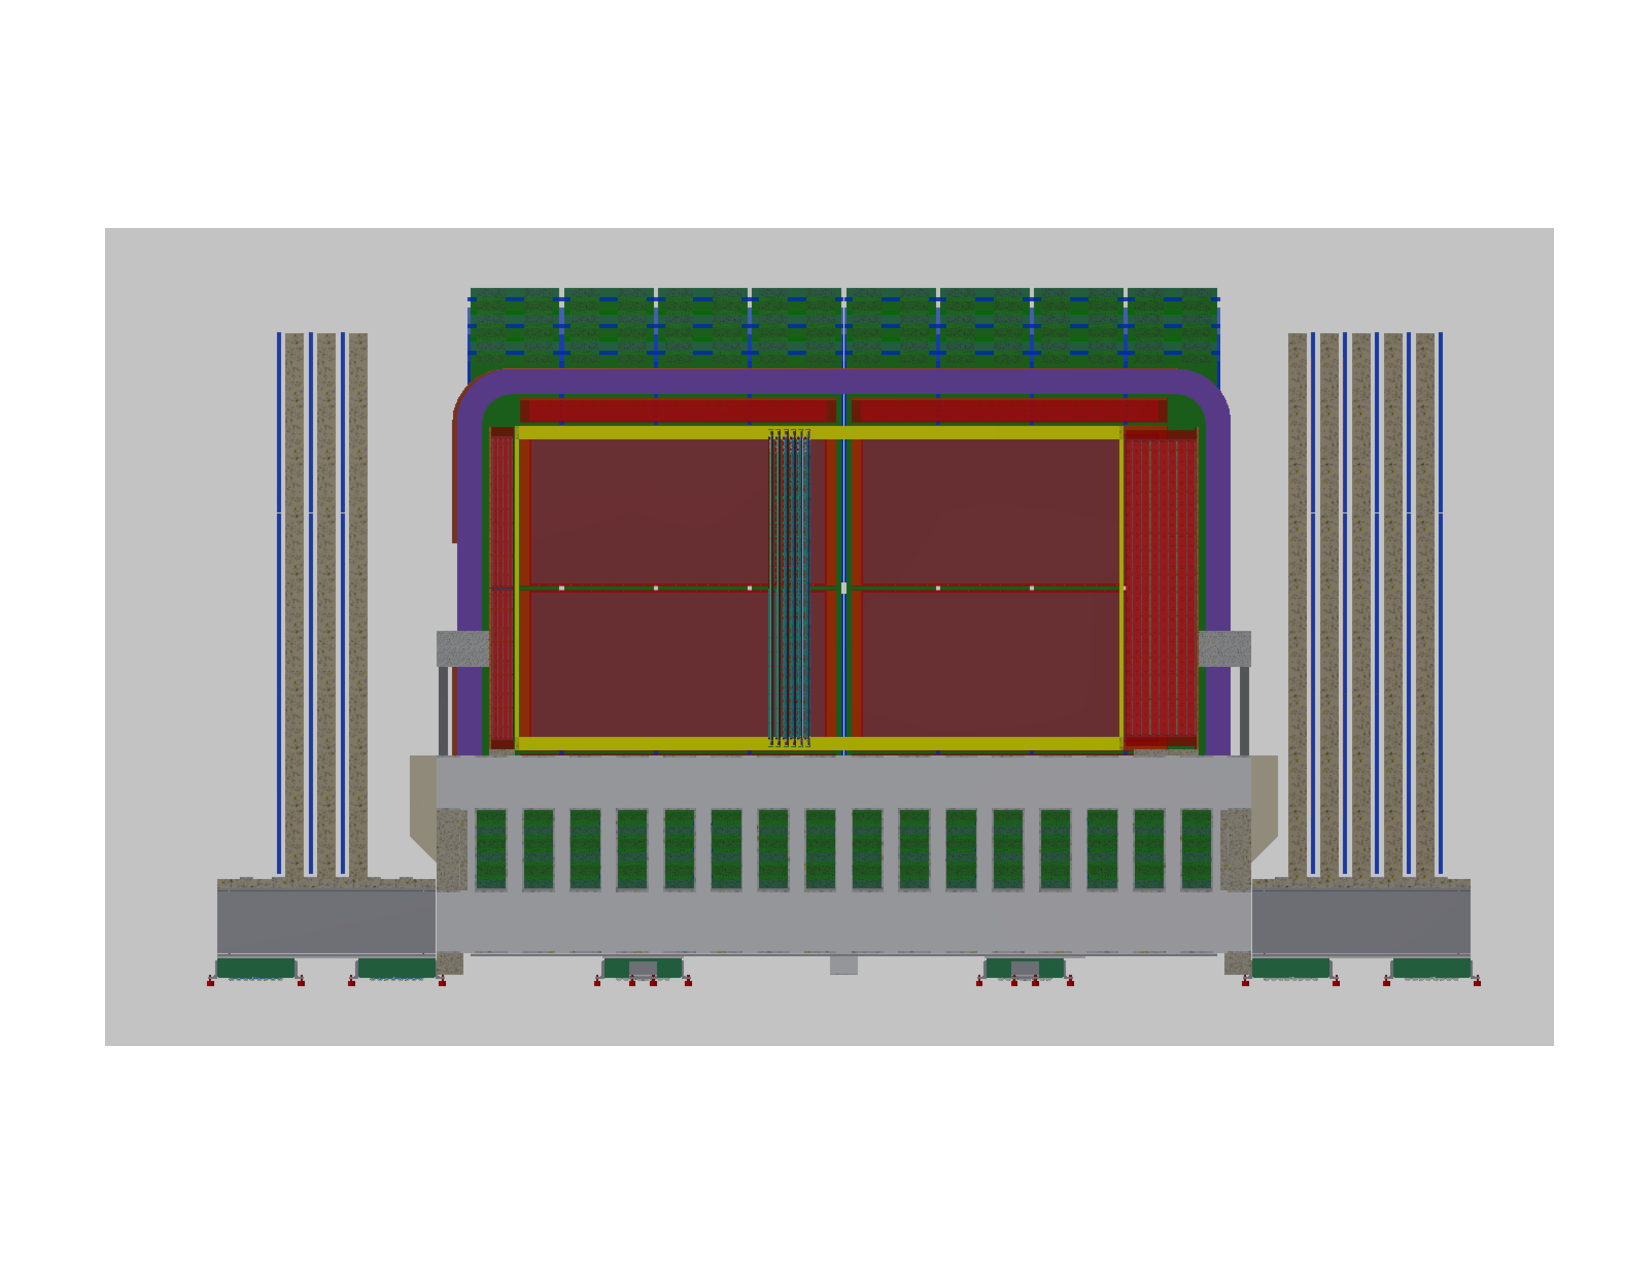
\includegraphics[width=3.0in,angle=90]{ECAL_gaps}
\end{cdrfigure}


\section{Dipole Magnet} 
\label{sec:nd-nnd-dipole}

The STT and ECAL modules will reside inside a 0.4-T dipole 
magnet for the measurement of particle momentum and charge. 
The magnet will have inner dimensions (inside the coils) 
4.5-m wide $\times$ 4.5-m high $\times$ 8.0-m long. The 
magnet 
%is modeled after the CERN 
%UA1 magnet with 
has four vertical Al coils, stacked horizontally, producing a horizontal magnetic 
field. The return yoke will be divided into two halves along the 
longitudinal center line to allow the magnet to be opened to service the
detector inside, as shown in Figure~\ref{fig:STT_schematic}. 
Each half yoke will be built
from eight ``C'' sections, and the thickness of the 
magnet steel will be 60~cm, consisting of 6
$\times$ 10-cm-thick plates. The magnet power requirement with Al coils is $\sim 2.4$~MW,
corresponding to 6~kA at 400~V. The water flow required for cooling is 20~l/s.
The Dipole Magnet specifications are shown in Table~\ref{tab:Magnet_specs}.

The momentum resolution is dominated by multiple scattering in the STT. The momentum resolution is, therefore, given by 
$\delta p/p = 0.053/\sqrt(LX_0)B$. For B = 0.4T, L = 3m, and $X_0 = 4$m, the
expected momentum resolution is $\sim 3.8\%$. 



\begin{cdrtable}[Dipole Magnet specifications]{ll}{Magnet_specs}{Dipole Magnet specifications}
Item&Specification \\ \toprowrule
Inner Dimensions & 4.5m x 4.5m x 8.0m \\ \colhline
Magnetic Field & 0.4 T \\ \colhline
Number of ``C'' Sections & 16 \\ \colhline
Thickness of Steel in the ``C'' Sections & 60cm \\ \colhline
Mass per ``C'' Section & 60 tonnes \\ \colhline
Number of Coils & 4 \\ \colhline
Mass per Coil & 40 tonnes \\ \colhline
Magnet Current & 6 kA \\ \colhline
Magnet Voltage & 400 V \\ \colhline
Magnet Power Requirements & 2.4 MW \\ \colhline
Water Flow for Cooling & 20 l/s \\\end{cdrtable}

\section{Muon Identifier}
\label{sec:nd-nnd-muid}

%\fixme{Lots of repetition here; can we just say 'like the LArTPCT MuID except for these differences...?}
%I would rather have the repetition so that it is a stand-alone section. BL}
The sides and ends of the dipole magnet will be instrumented
with a muon identifier
detector (MuID) that will distinguish muons from hadrons by their ability 
to penetrate the iron without showering or interacting.
The MuID will consist of 432 RPC modules
interspersed between 2 $\times$ 10-cm-thick steel plates of the 
dipole magnet and between 20-cm-thick steel plates at the upstream and
downstream ends of the magnet. 
The MuID is only meant to provide %the 
identification of the 
muon; the muon momentum %itself 
will be measured by the STT inside the 
magnetic field. A schematic drawing of the MuID 
interspersed in the magnet steel is shown in Figure~\ref{fig:FGT_MuID}.

The nominal dimensions of all RPC modules will be 1~m $\times$ 2~m with
active areas of 196cm x 96cm. Each
module has 256 X strips
at 7.65 mm pitch and 128 Y strips at 7.5 mm pitch. The modules
will be grouped into trays containing 6 modules each, and the trays will
be sufficiently wide to allow overlapping modules. 
The end-RPC trays have dimensions of 2m x 6m, and there are 3 trays per plane.
The downstream end has 5 planes, corresponding to 15 trays and 90 RPC modules.
The upstream end has 3 planes, corresponding to 9 trays and 54 RPC modules.
The vertical barrel-RPC trays have dimensions of 2.5m x 4m, 2.8m x 4m, and
3.1m x 4m for the inner, middle, and, outer planes, respectively, corresponding
to 24 trays and 144 RPC modules. The horizontal
barrel-RPC trays have dimensions of 2.2m x 4m, 2.5m x 4m, and
2.8m x 4m for the inner, middle, and, outer planes, respectively, 
corresponding to 24 trays and 144 RPC modules. Overall, there are a total of
72 trays, 432 RPC modules, and 165,888 strips and electronic channels. 

The downstream MuID will contain 5 steel planes of 
overall dimension
6 x 6 x 0.2 m$^3$ (283.5 tonnes)
and 5 RPC planes, while the upstream MuID will contain 3 steel
planes (170.1 tonnes) of dimension 6 x 6 x 0.2 m$^3$ and 3 RPC planes. The barrel MuID will contain
24 planes (3 layers x 8 sides) of RPCs. The RPCs will have a total thickness 
of 15 mm and a gap width of 2 mm. One possible gas mixture would be composed, for example,
of Ar (75\%), tetraflouroethane (20\%), isobutane (4\%),
and sulphurhexaflouride (1\%). 
A schematic drawing of an RPC is shown in Figure~\ref{fig:FGT_RPC}, while
Figure~\ref{fig:RPC_Tray} shows a schematic drawing of an end-RPC tray,
and Figure~\ref{fig:FGT_RPC} shows a schematic drawing of an RPC module.
MuID specifications are shown in Table~\ref{tab:MID_specs}.

\begin{cdrfigure}[Schematic drawing of a magnet half-assembly]{FGT_MuID}{Schematic drawing of a magnet half-assembly, 
showing the the MuID interspersed in the magnet steel}
%\includegraphics[width=5in,angle=90]{Magnet_Half_Assembly}
\end{cdrfigure}


\begin{cdrfigure}[Schematic drawing of an end-RPC tray]{RPC_Tray}{Schematic drawing of an end-RPC tray,
consisting of six RPC modules of dimension 1m $\times$ 2m}
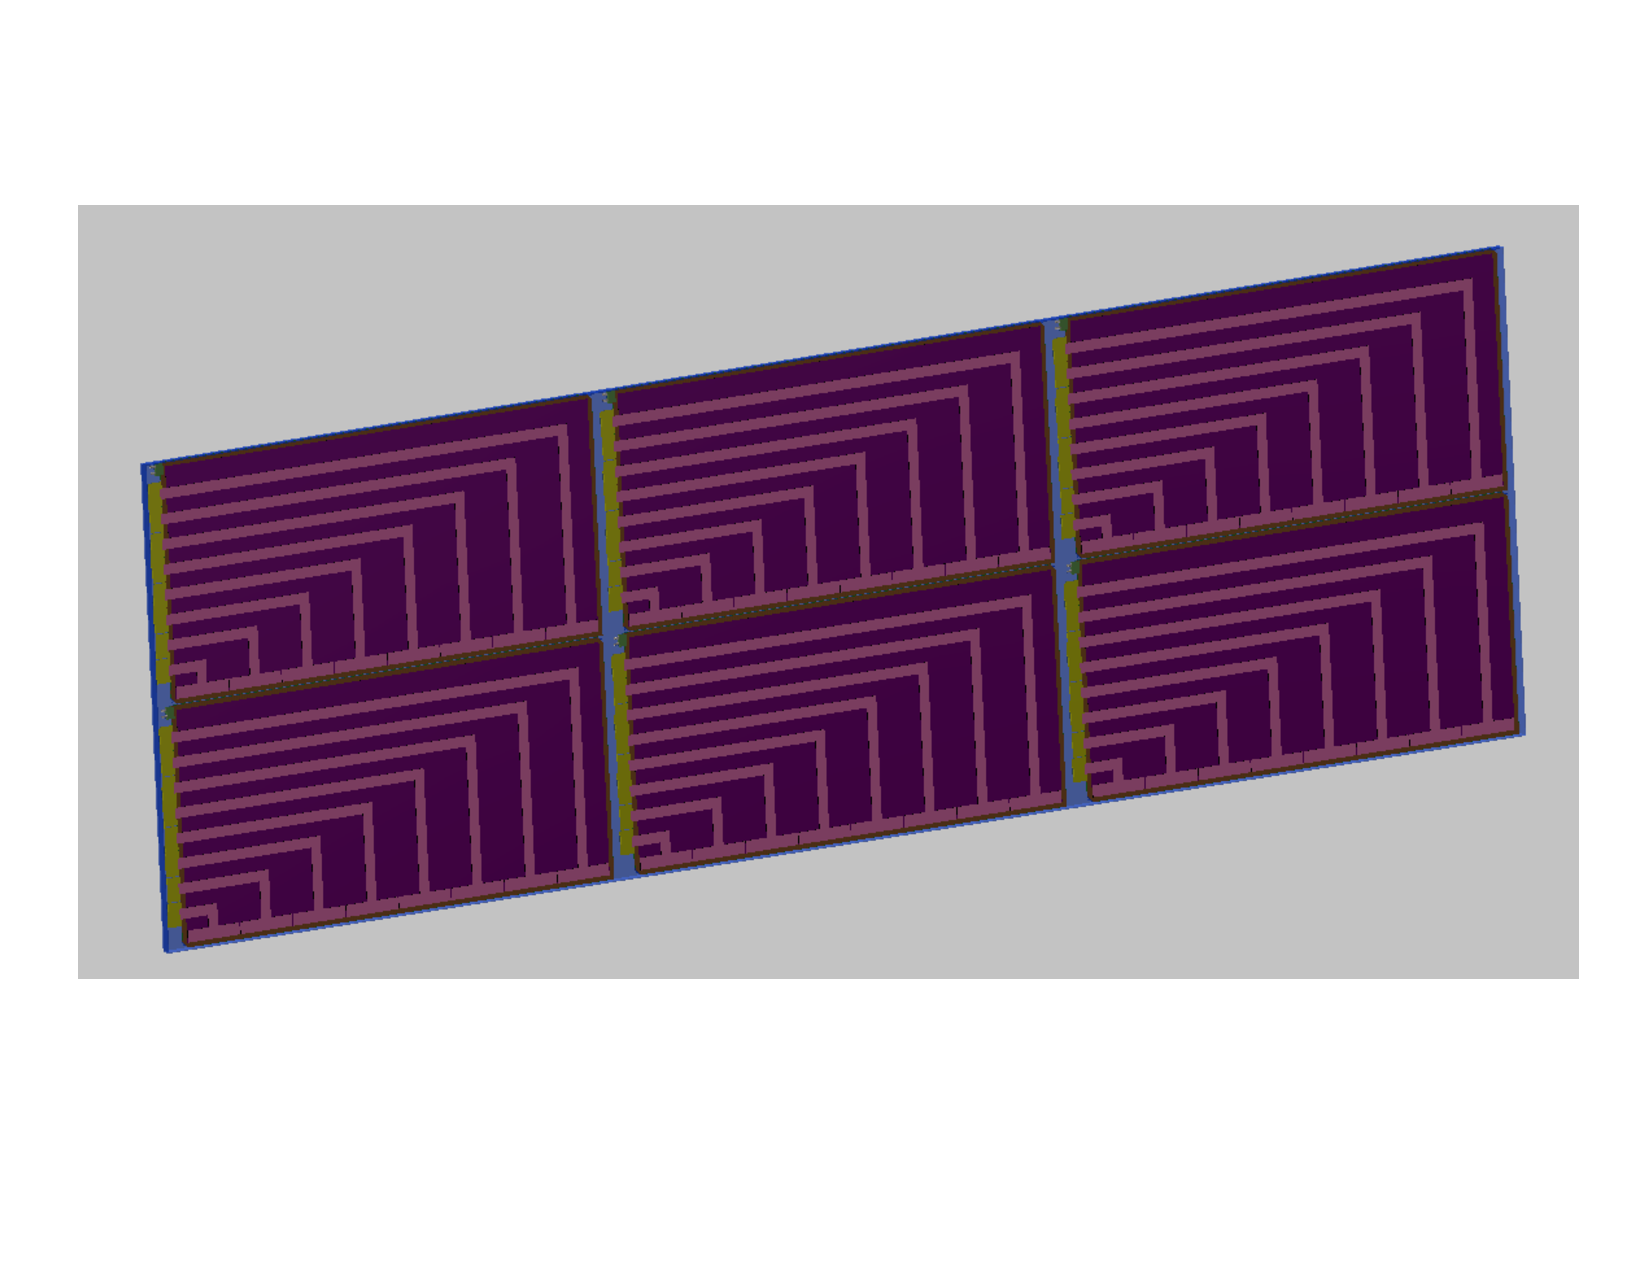
\includegraphics[width=3in,angle=90]{RPC_Tray}
\end{cdrfigure}


\begin{cdrfigure}[Schematic drawing of an RPC]{FGT_RPC}{Schematic drawing of an RPC}
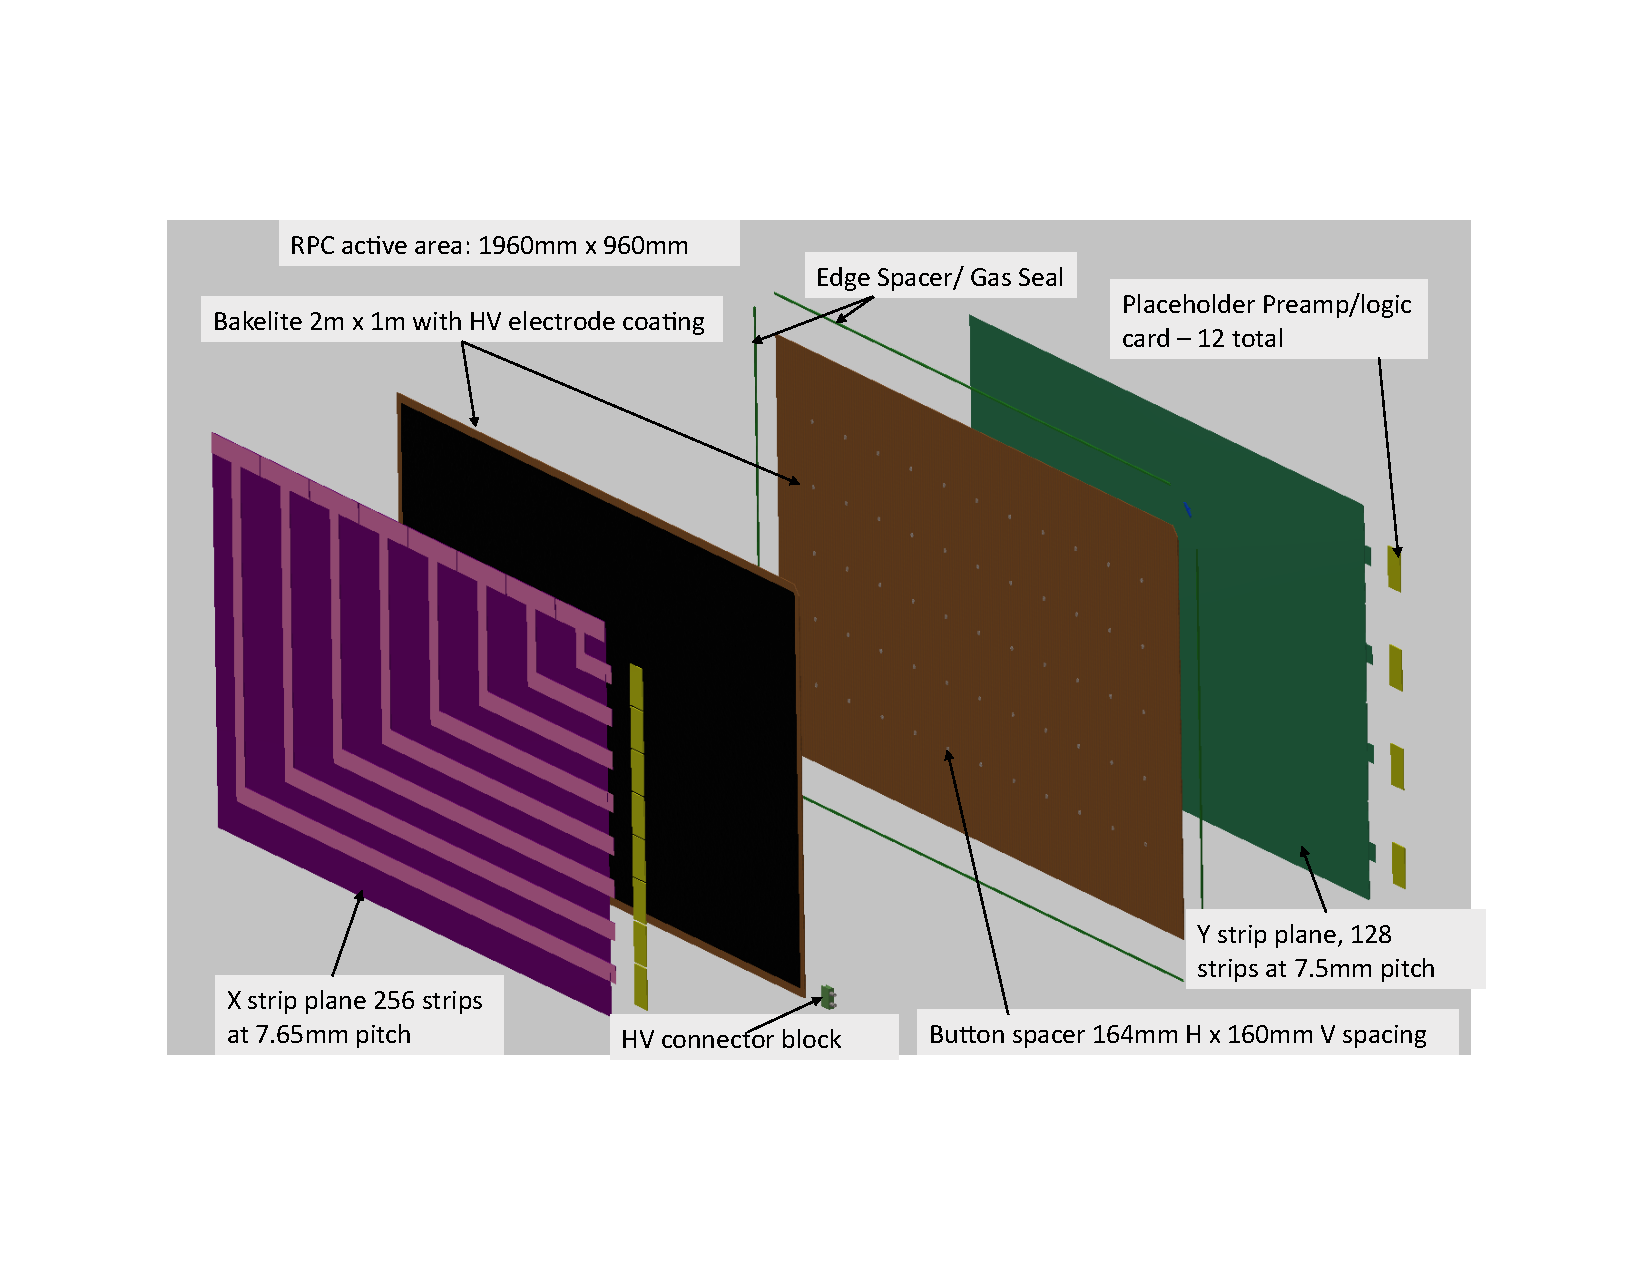
\includegraphics[width=3in,angle=90]{RPC_Detail}
\end{cdrfigure}



\begin{cdrtable}[MuID specifications]{ll}{MID_specs}{MuID specifications}
Item&Specification  \\ \toprowrule
Number of Barrel RPC Trays of Dimension 2.2m $\times$ 4m & 8 \\ \colhline
Number of Barrel RPC Trays of Dimension 2.5m $\times$ 4m & 16 \\ \colhline
Number of Barrel RPC Trays of Dimension 2.8m $\times$ 4m & 16 \\ \colhline
Number of Barrel RPC Trays of Dimension 3.1m $\times$ 4m & 8 \\ \colhline
Number of END RPC Trays of Dimension 2m $\times$ 6m & 24 \\ \colhline
Total Number of RPC Trays & 72 \\ \colhline
Total Number of RPC Modules & 432 \\ \colhline
Mass of Downstream Steel Planes & 283,500 kg \\ \colhline
Mass of Upstream Steel Planes & 170,100 kg \\ \colhline
RPC Thickness & 1.5cm \\ \colhline
Number of 7.65mm Pitch X Strips per Module & 256 \\ \colhline
Number of 7.5mm Pitch Y Strips per Module & 128 \\ \colhline
Total Number of RPC Strips and Electronics & 165,888 \\
\end{cdrtable}

\section{FGT Instrumentation}
\label{sec:nd-nnd-intrumentation}

The instrumentation includes readout electronics for the subdetectors
and the slow control of the \fixme{which?} subdetector, involving monitoring the humidity, 
temperature, gas pressure, etc.
There is considerable synergy in the information \fixme{of what type} gathered in the STT, ECAL and MuID.
Both the STT and ECAL are required to measure the total charge and the time associated with a 
given hit. The MuID RPCs are required to provide the position and time associated with 
a traversing track. Similarly, the slow control of the subdetectors
share many features. 
A brief description of the subdetector instrumentation is presented below, while
Table~\ref{tab:elect_ch} summarizes the number of electronics channels for each of the
three detector systems. \fixme{detector system = subdetector?}

\fixme{add something here about the cooling water flow and voltage and current monitoring; you have no information in the sections, so they should be removed.}


\begin{cdrtable}[Number of electronics channels for each of the
three detector systems]{ll}{elect_ch}{The number of electronics channels for each of the
three detector systems}
Detector&Number of Electronics Channels\\ \toprowrule
STT & 215,040 \\  \colhline
ECAL & 52,224 \\  \colhline
MuID & 165,888 \\
\end{cdrtable}

\subsection{Readout Electronics} % for the FGT}

The electronics for the three subsystems, STT, MuID, and ECAL, are all fast systems, 
i.e. all of the signals are fast in the few to 10 nanosecond range.  The STT output has 
about 10 nanosecond rise time with a total integrated charge of about of about 100 
electrons per centimeter.  The gain of the STT drift tubes are typically $10^4$ to $10^6$, 
so the integrated charge is  $10^6$ to $10^8$ electrons collected over a time interval of 
$\sim 100$ns.  The MuId system contains Resistive Plate Chambers (RPC) that can operate 
in either the streamer mode or avalanche mode; the difference is that the avalanche mode 
is proportional to the deposited charge, while the streamer mode is not proportional to 
the deposited charge.  The rise time of the RPC signal is a few nanoseconds and is 
collected immediately, and the collected charge can be large up to 100 pC.  The ECAL 
signals come from an SiPM (silicon photomultiplier) that converts the light from the 
scintillator strips to an electronic signal. The deposited charge in the scintillator 
will give rise to $10^3$ to $10^5$ photoelectrons.  The gain of an SiPM is $\sim 10^6$ and 
has a rise time of a few nanoseconds, so the total charge can be $> 100$ pC. As these 
three systems all have gain and are fast, our hope is that it might be possible to have a 
common electronics system.  

The requirements for each system are very similar: a fast output, an ADC on each channel, 
and a TDC on each channel.  An additional requirement for the STT straw tubes is that it 
is desirable to wave-form digitize the analog signal to enhance the ability to separate 
the ionization signal from the transition radiation signal.  The channel count for the 
three systems are: STT 215000 channels, MuID 165000 channels, and ECAL 52224 channels, 
for a total channel count  of 433152 channels.   Most available electronic systems from 
existing experiments don’t quite meet these requirements or are too expensive to implement 
for our channel count.  We have allocated \$50/channel.  Recently, we have been made aware 
of a new ASIC development for an upgrade to the ATLAS muon system at the LHC.  The 
development comes from G. DeGeronimo at BNL.  A schematic of the chip(VMM2) is shown in 
Figure \ref{VMM2}.  It handles 64 channels and produces both fast ADC and TDC outputs.
It has been fabricated and tested and should be ready by 2017, long before our needs.  
The VMM2 features are the following:
\begin{itemize}
\item Front-end Electronics (ASIC)
\item more than 2.3 million channels total
\item operate with both charge polarities
\item sensing element capacitance 10-200 pF
\item charge measurement up to 2 pC at $< 1$ fC RMS
\item time measurement $\sim 100$ ns at $< 1$ ns RMS
\item trigger primitives, neighbor logic
\item low power, programmable
\end{itemize}
We will explore the VMM2 chip as our first option for the readout.  


\begin{cdrfigure}[A schematic drawing of the VMM2 circuit]{VMM2}{A schematic drawing of the VMM2 circuit}
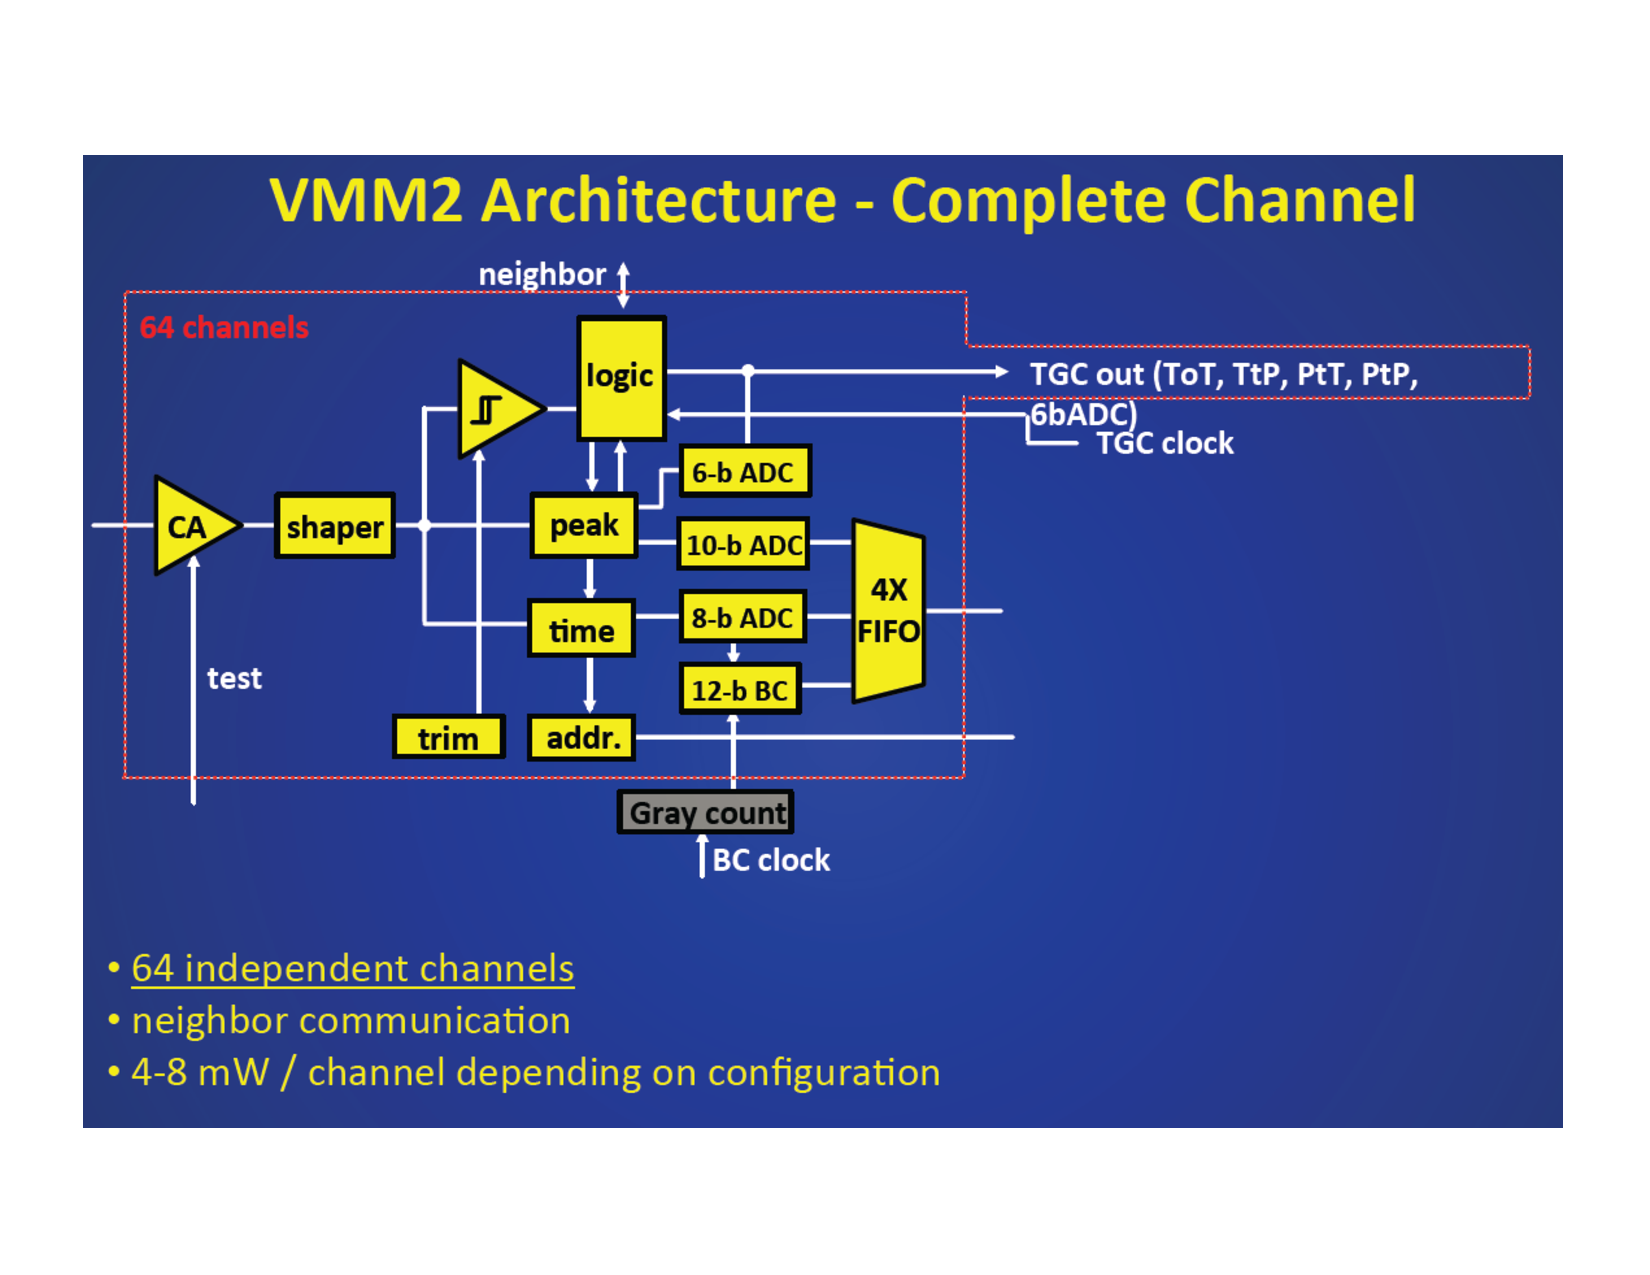
\includegraphics[width=5in,angle=0]{VMM2}
\end{cdrfigure}


\subsection{Data Acquisition} % Nearsite Neutrino Detector (NND) DAQ}

The Nearsite Neutrino Detector Data Acquisition system (NND-DAQ) collects raw data from 
each %near 
detector subsystem in the Near Neutrino Detector (NND) and connects to the Near 
Detector System DAQ (NDS-DAQ), described in Chapter~\ref{ch:nd-gdaq}, via Gigabit Ethernet. A block diagram of the NND-DAQ is
shown in Figure~\ref{fig:DAQ_NND}.
Similar to the NDS-DAQ, the NND-DAQ will mainly consist 
of a scalable back-end computer array, inter-connected to the individual Near Neutrino 
Detector DAQs via Gigabit Ethernet and specialized electronics modules for trigger 
processing and clock synchronization. It interfaces to the NDS Master DAQ (NDS-MDAQ),
described in Section~\ref{sec:nd-master-daq}, for 
run control and global \fixme{still want `global'?} data collection. It will also have its own local run-control setup, 
consisting of a number of desktop workstations to allow independent local runs that include 
nearsite neutrino detectors \fixme{`detectors' or `detector systems'?} only, useful during detector commissioning, calibration runs, 
stand-alone cosmic runs or other runs where the beam is stopped or not needed.

The quantity of computers required for the back-end system is highly dependent on the 
number of channels and expected data rates of the individual neutrino detectors. Based on 
T2K Near Detector DAQ experience\fixme{ref?}, one back-end computer should be able to handle 
approximately 3,000 channels for sustainable and continuous runs. Assuming a total of 
430,000 channels for all neutrino detectors \fixme{?} combined, about 150 back-end computers would be 
needed.

Trigger signals from each neutrino detector \fixme{?} will be collected and pre-processed by a 
trigger electronics module, similar in design to the global \fixme{?}  trigger or master clock modules 
of the NDS-DAQ design. Depending on the run mode, this module could feed local trigger 
decisions to the detector DAQs for data collection, or it could forward global  \fixme{?} triggers 
from the NDS-DAQ or higher levels to the neutrino detector DAQs.  A slave-clock electronics 
module, similar to the master-clock module in the NDS-DAQ, distributes clock- and 
time-synchronization signals from the NDS-DAQ to all neutrino detectors  \fixme{?} .


\begin{cdrfigure}[A block diagram of the Near Neutrino Detector DAQ]{DAQ_NND}{A block diagram of the Near Neutrino Detector DAQ (NND-DAQ)}
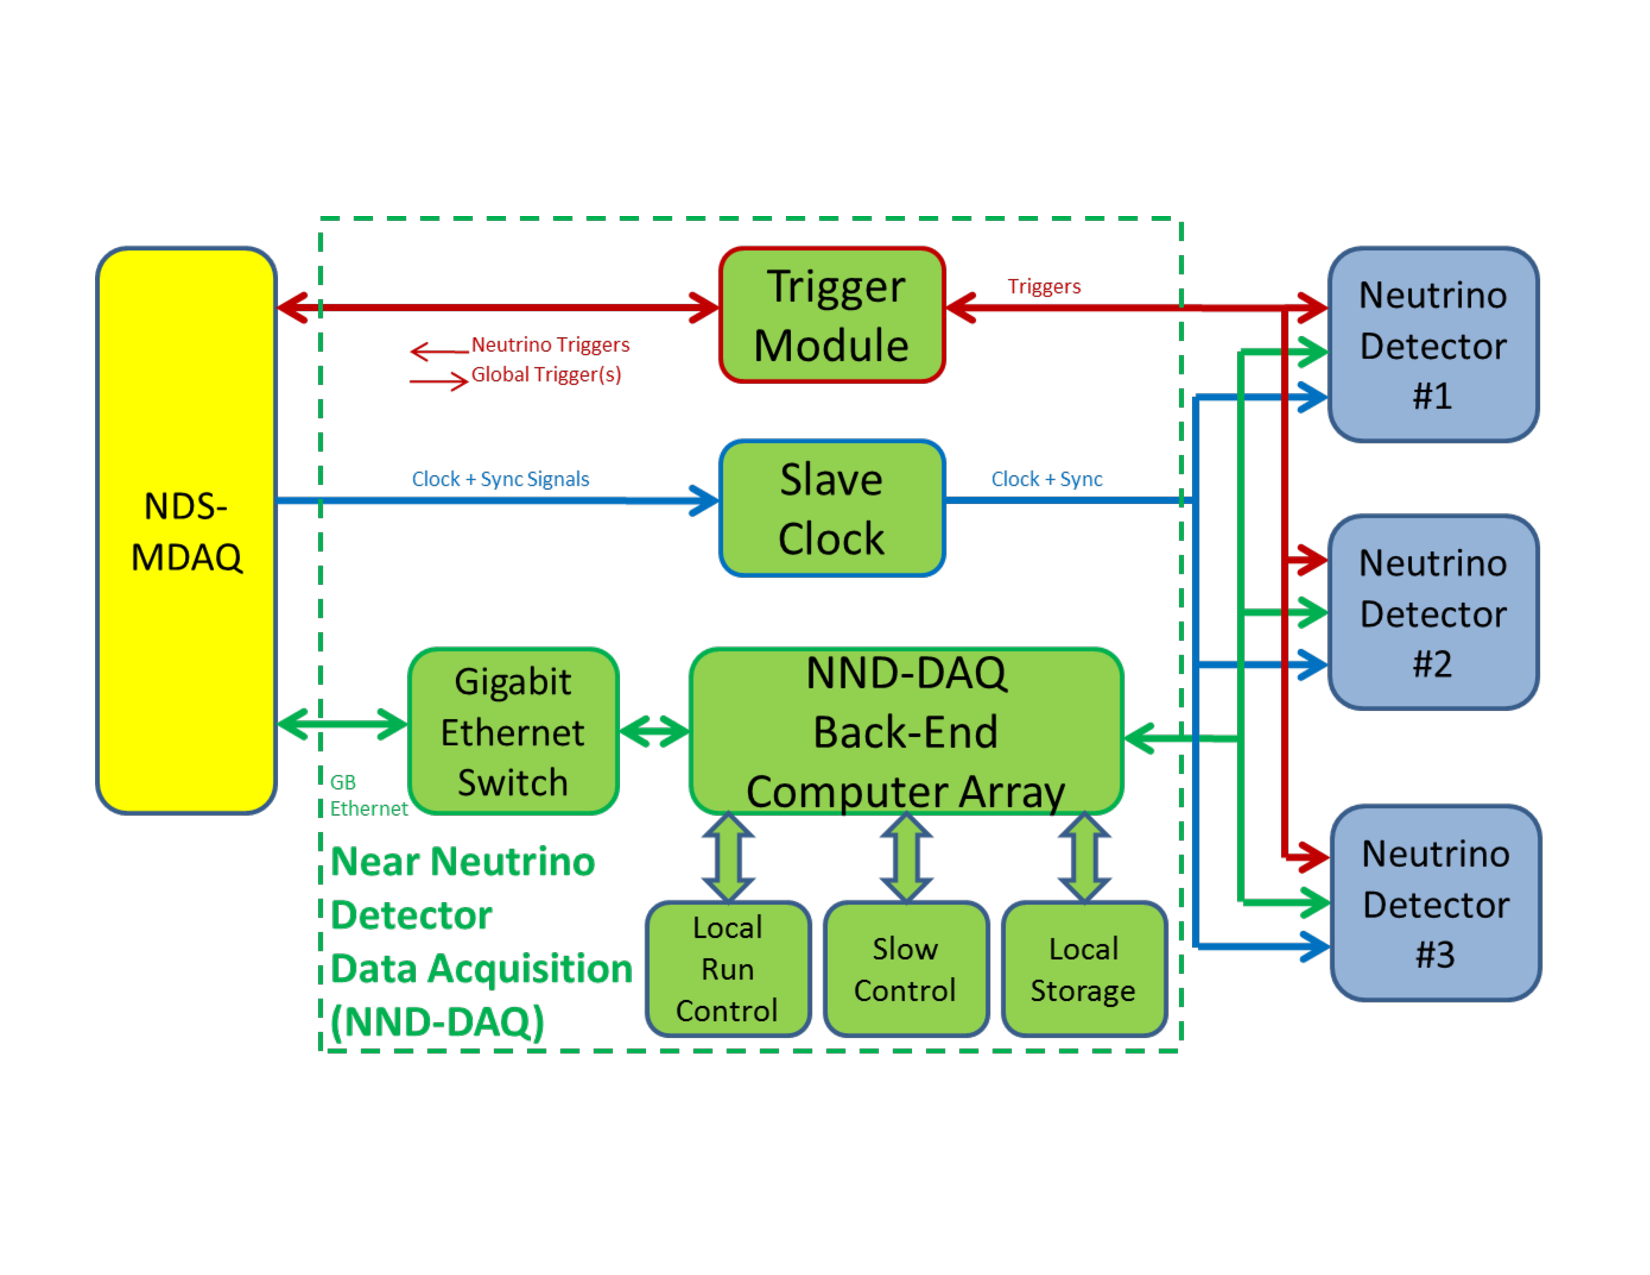
\includegraphics[width=6in,angle=0]{DAQ_NND}
\end{cdrfigure}


\subsection{Humidity and Temperature Monitoring } % in the STT, ECAL, MuID, and Magnet}

Humidity is inimical to all sub-detectors in the FGT. To maintain a low-level of 
humidity and to maintain a desired temperature, both STT and ECAL sub-detectors
will have dry nitrogen circulating within their outer layers. A similar arrangement 
might be made for the RPCs as well. Furthermore, magnet coils are cooled by water, 
while the magnet yokes are instrumented with RPCs. Thus, a continuous control of 
humidity in all these detectors is needed.
Just as humidity, temperature must be continuously monitored in all of the sub-detectors.

\subsection{Gas Leak Monitoring in the STT and MuID}

Gas-leaks need to be monitored in the STT and MuID.
The STT will employ Xe gas, which is expensive and, hence, will be recirculated. It is 
most essential to ensure that Xe is not leaking. The requirement for leaks is less 
stringent for the RPC. 

\subsection{Cooling-Water Flow Monitoring in the Magnet}

The water flow (pressure gradient) must be continuously monitored.  \fixme{Add more or remove section, I'd say and . AH}

\subsection{Monitoring Voltage and Current}

All power sources instrumenting the FGT and its readout need to be monitored for 
appropriate voltage and current.

\fixme{Add more or remove section, I'd say and . AH}

%\section{Liquid Argon TPC Alternative Design}
%\label{sec:nd-nnd-lar-tpc-alt}

%\section{Pressurized GAS TPC Alternative Design}
%\label{sec:nd-nnd-gas-tpc-alt}





